\section{Используемые технологии и аппаратная платформа}


\subsection{Язык программирования С++}

С++ является языком программирования общего назначения. Естественная для него область
применения - системное программирование, понимаемое в широком смысле этого слова. Кроме того,С++ успешно используется во многих областях приложения, далеко выходящих за указанные рамки.Реализации С++ теперь есть на всех машинах, начиная с самых скромных микрокомпьютеров - до самых больших супер-ЭВМ, и практически для всех операционных систем. Поэтому книга дает лишь описание собственно языка, не объясняя особенности конкретных реализаций, среды программирования или библиотек.

С++ - язык общего назначения и задуман для того, чтобы настоящие программисты получили
удовольствие от самого процесса программирования. За исключением второстепенных деталей он содержит язык С как подмножество. Язык С расширяется введением гибких и эффективных средств, предназначенных для построения новых типов. Программист структурирует свою задачу, определив новые типы, которые точно соответствуют понятиям предметной области задачи. Такой метод построения программы обычно называют абстракцией данных. Информация о типах содержится в некоторых объектах типов, определенных пользователем. С такими объектами можно работать надежно и просто даже в тех случаях, когда их тип нельзя установить на стадии трансляции. Программирование с использованием таких объектов обычно называют объектно-ориентированным. Если этот метод применяется правильно, то программы становятся короче и понятнее, а сопровождение их упрощается.

Ключевым понятием С++ является класс. Класс - это определяемый пользователем тип. Классы обеспечивают упрятывание данных, их инициализацию, неявное преобразование пользовательских типов, динамическое задание типов, контролируемое пользователем управление памятью и средства для перегрузки операций. В языке С++ концепции контроля типов и модульного построения программ реализованы более полно, чем в С. Кроме того, С++ содержит усовершенствования, прямо с классами не связанные: символические константы, функции-подстановки, стандартные значения параметров
функций, перегрузка имен функций, операции управления свободной памятью и ссылочный тип. В С++ сохранены все возможности С эффективной работы с основными объектами, отражающими аппаратную "реальность" (разряды, байты, слова, адреса и т.д.). Это позволяет достаточно эффективно реализовывать пользовательские типы.

Как язык, так и стандартные библиотеки С++ проектировались в расчете на переносимость. Имеющиеся реализации языка будут работать в большинстве систем, поддерживающих С. В программах на С++ можно использовать библиотеки С. Большинство служебных программ, рассчитанных на С, можно использовать и в С++.

Развитие языка С++ происходило на базе языка С, и, за небольшим исключением, С был сохранен в качестве подмножества C++. Базовый язык С был спроектирован таким образом, что имеется очень тесная связь между типами, операциями, операторами и объектами, с которыми непосредственно работает машина, т.е. числами, символами и адресами. За исключением операций new, delete и throw, а также проверяемого блока, для выполнения операторов и выражений С++ не требуется скрытой динамической аппаратной или программной поддержки.

В С++ используется та же (или даже более эффективная) последовательность команд для вызова функций и возврата из них, что и в С. Если даже эти довольно эффективные операции становятся слишком дорогими, то вызов функции может быть заменен подстановкой ее тела, причем сохраняется удобная функциональная запись безо всяких расходов на вызов функции.

Первоначально язык С задумывался как конкурент ассемблера, способный вытеснить его из основных и наиболее требовательных к ресурсам задач системного программирования. В проекте С++ были приняты меры, чтобы успехи С в этой области не оказались под угрозой. Различие между двумя языками прежде все состоит в степени внимания, уделяемого типам и структурам. Язык С выразителен и в то же время снисходителен по отношению к типам. Язык С++ еще более выразителен, но такой выразительности можно достичь лишь тогда, когда типам уделяют большое внимание. Когда типы объектов известны, транслятор правильно распознает такие выражения, в которых иначе программисту пришлось бы записывать операции с утомительными подробностями. Кроме того, знание типов позволяет транслятору обнаруживать такие ошибки, которые в противном случае были бы выявлены только при тестировании. Отметим, что само по себе использование строгой типизации языка для контроля параметров функции, защиты данных от незаконного доступа, определения новых типов и операций не влечет дополнительных расходов памяти и увеличения времени выполнения программы.

В проекте С++ особое внимание уделяется структурированию программы. Это вызвано увеличением размеров программ со времени появления С. Небольшую программу (скажем, не более 1000 строк) можно заставить из упрямства работать, нарушая все правила хорошего стиля программирования. Однако, действуя так, человек уже не сможет справиться с большой программой. Если у вашей программы в 10 000 строк плохая структура, то вы обнаружите, что новые ошибки появляются в ней так же быстро, как удаляются старые. С++ создавался с целью, чтобы большую программу можно было
структурировать таким образом, чтобы одному человеку не пришлось работать с текстом в 25000 строк. В настоящее время можно считать, что эта цель полностью достигнута.

Существуют, конечно, программы еще большего размера. Однако те из них, которые действительно используются, обычно можно разбить на несколько практически независимых частей, каждая из которых имеет значительно меньший упомянутого размер. Естественно, трудность написания и сопровождения программы определяется не только числом строк текста, но и сложностью предметной области. Так что приведенные здесь числа, которыми обосновывались наши соображения, не надо воспринимать слишком серьезно.

К сожалению, не всякую часть программы можно хорошо структурировать, сделать независимой от аппаратуры, достаточно понятной и т.д. В С++ есть средства, непосредственно и эффективно представляющие аппаратные возможности. Их использование позволяет избавиться от беспокойства о надежности и простоте понимания программы. Такие части программы можно скрывать, предоставляя надежный и простой интерфейс с ними.

Естественно, если С++ используется для большой программы, то это означает, что язык используют группы программистов. Полезную роль здесь сыграют свойственные языку модульность, гибкость и строго типизированные интерфейсы. В С++ есть такой же хороший набор средств для создания больших программ, как во многих языках. Но когда программа становится еще больше, проблемы по ее созданию и сопровождению перемещаются из области языка в более глобальную область программных средств и управления проектом \cite{StroustrupCpp}.


\subsection{Система компиляции}

Исторически компиляторы не функционируют изолированно, а интегрированы в сложные инструментальные цепочки (тулчейны). На практике пользователи редко запускают компилятор напрямую: такие программы, как GCC, Clang или ICC, представляют собой драйверы, координирующие выполнение множества вспомогательных инструментов, включая препроцессор, ассемблер, компоновщик и другие компоненты. Хотя конечной целью является преобразование исходного кода в исполняемый файл, этот процесс требует согласованной работы всего инструментального набора.

Термин "компилятор Clang" в обиходе часто относится не только к самому компилятору, но и к LLVM Toolchain — обширной экосистеме взаимосвязанных компонентов и библиотек. Для понимания принципов работы компилятора необходимо учитывать его место в этой структуре. Даже в изолированном рассмотрении компилятор выполняет не только оптимизацию кода, но и ряд других задач, что подчеркивает важность понимания архитектуры его внутренних компонентов.

Инструментальная среда разработки включает множество вспомогательных средств, таких как ассемблеры, компоновщики, отладчики и профилировщики, которые формируют общий ландшафт работы с компиляторами. Хотя подробное рассмотрение каждого из них выходит за рамки данного исследования, представленный анализ ключевых аспектов их взаимодействия имеет значение не только для разработчиков компиляторов, но и для специалистов, использующих их в практической деятельности.

\begin{figure}[H]
	\centering
	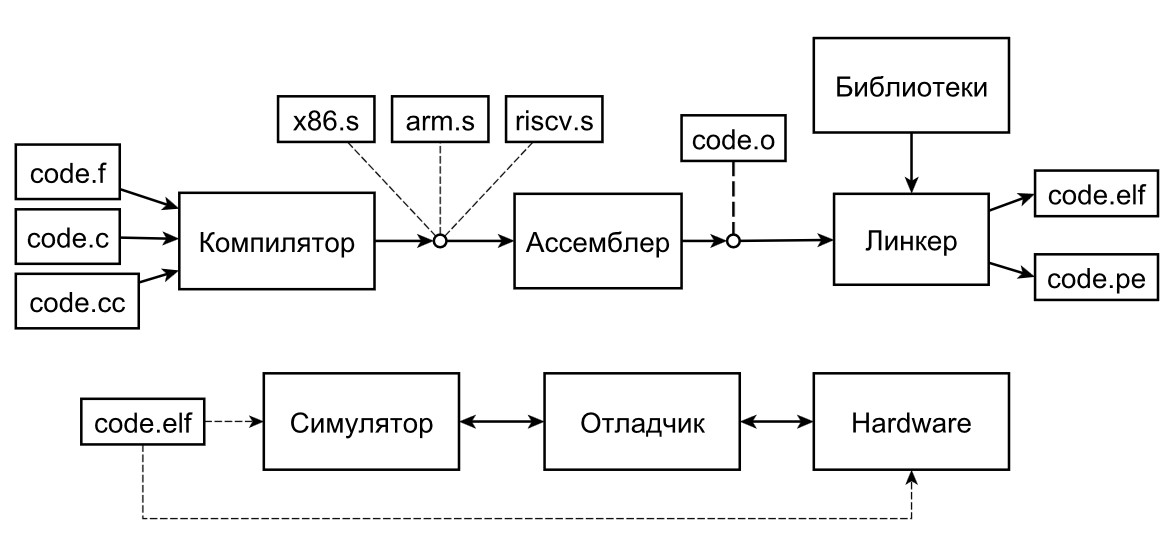
\includegraphics[scale=0.77]{tul.jpg}
	\caption{Упрощенная схема системы компиляции}
	\label{fig:tulchain}
\end{figure}

Упрощённая схема процесса компиляции представлена на рисунке \ref{fig:tulchain}. Ключевыми компонентами системы являются компилятор, ассемблер и линкер. Результатом работы системы является исполняемый файл (бинарный файл, содержащий машинный код). Полученный файл может быть отлажен и запущен как на физическом устройстве, так и в среде симуляции. Использование симулятора особенно актуально при кросс-компиляции, когда целевая архитектура отличается от архитектуры системы, на которой выполняется компиляция.

Таким образом, программа-драйвер объединяет три ключевых компонента: компилятор, ассемблер и линкер. Далее рассмотрим каждый из этих элементов более подробно.

Компилятор является центральным и наиболее сложным компонентом системы компиляции. Как видно из рисунка \ref{fig:tulchain}, его основная функция заключается в преобразовании исходного кода, написанного на высокоуровневом языке программирования, в эквивалентный код на языке ассемблера. 

Большинство современных компиляторов функционируют в соответствии с принципом, известным как "правило as-if" (as-if rule). Согласно этому принципу, компилятор может применять любые оптимизации при условии, что наблюдаемое поведение корректно исполняемой программы остаётся эквивалентным поведению, которое предполагал программист при написании исходного кода.

Ключевым аспектом данного правила является то, что оно гарантирует сохранение семантики только для корректных программ. В случае возникновения ситуаций с неопределённым поведением (undefined behavior), таких как знаковое целочисленное переполнение, компилятор вправе считать такие сценарии невозможными и не учитывать их при оптимизации.

С архитектурной точки зрения компилятор состоит из фронтенда (frontend) и бэкенда (backend). Фронтенд занимается анализом исходного кода и построением промежуточного представления программы, тогда как бэкенд выполняет оптимизацию этого представления и генерацию машинного кода. Использование англоязычных терминов "фронтенд" и "бэкенд" является общепринятой практикой, поскольку эти понятия прочно укоренились не только в компиляторостроении, но и в других областях компьютерных наук (хотя и с иной семантикой), а попытки их буквального перевода приводят к громоздким и менее точным формулировкам. В некоторых реализациях выделяют дополнительный компонент - мидленд ( middle-end), ответственный исключительно за оптимизацию, оставляя за бэкендом только финальную кодогенерацию. Однако такая терминология не получила широкого распространения в индустрии, поэтому в дальнейшем изложении мы будем рассматривать бэкенд как единый модуль, включающий как оптимизатор, так и генератор кода.

Термин "ассемблер" имеет два основных значения в контексте систем программирования. Во-первых, это язык ассемблера - низкоуровневый язык программирования, специфичный для конкретной компьютерной архитектуры. Во-вторых, это программа-ассемблер, выполняющая трансляцию исходного кода на языке ассемблера в объектный код.

Объектный код представляет собой промежуточное представление машинных инструкций, где команды процессора уже закодированы в двоичной форме, но ещё не готовы к непосредственному исполнению. Такой код требует дополнительной обработки компоновщиком (линкером) для формирования окончательного исполняемого файла.

В современных системах компиляции ассемблер может быть реализован как отдельная программа или интегрирован в компилятор. В последнем случае компилятор способен генерировать объектный код напрямую, минуя этап явного ассемблирования. Такая интеграция позволяет оптимизировать процесс трансляции и повысить общую производительность системы компиляции.

Возникает закономерный вопрос: зачем нужен язык ассемблера, если компилятор может генерировать объектный код напрямую? Это обусловлено несколькими важными причинами.

Во-первых, ассемблерный код значительно удобнее для анализа и отладки по сравнению с бинарным представлением. При диагностике сложных проблем, особенно тех, которые слабо проявляются в отладочных сборках, работа с дизассемблированным кодом остаётся стандартной практикой.

Во-вторых, набор машинных инструкций современных процессоров гораздо шире, чем те, которые обычно генерирует компилятор. Многие специализированные команды (например, для работы с системными регистрами или управления аппаратными особенностями процессора) недоступны через высокоуровневые языки. В таких случаях (например, при разработке низкоуровневого ПО, включая операционные системы или драйверы) написание кода на ассемблере становится необходимым.

Таким образом, несмотря на возможность прямой генерации объектного кода, язык ассемблера сохраняет свою актуальность как для отладки, так и для низкоуровневого программирования.

Ещё один закономерный вопрос — зачем нужен объектный код, если можно сразу генерировать исполняемый файл? Основная причина кроется в необходимости раздельной компиляции. Практически все современные языки программирования поддерживают возможность компиляции отдельных модулей независимо друг от друга. Это особенно важно при работе с библиотеками — их код компилируется один раз, а затем многократно используется в разных проектах. Объектный файл как раз и служит таким промежуточным форматом, который сохраняет не только сам машинный код, но и всю необходимую для линкера информацию: таблицы символов, неразрешённые внешние ссылки, данные для отладки и другую метаинформацию. При этом в итоговом исполняемом файле большая часть этих данных становится ненужной — линкер уже разрешил все зависимости и создал единый исполняемый образ. Таким образом, объектный код выступает в роли универсального контейнера, который с одной стороны содержит всё необходимое для последующей компоновки, а с другой — позволяет избежать повторной компиляции одних и тех же модулей, значительно ускоряя процесс разработки.

Статическая линковка выполняется после ассемблирования. В простейшем случае достаточно передать линкеру (например, GNU ld) ваши объектные файлы вместе со стандартными библиотеками. Однако пути к этим библиотекам сильно зависят от параметров сборки: используются разные версии для 32-битного и 64-битного кода, различные ABI в рамках одной архитектуры и другие специфические варианты целевой платформы. Поэтому правильные пути к библиотекам обычно определяет драйвер компилятора на основе множества факторов, включая неочевидные системные настройки. Хотя эти пути можно вручную подсмотреть в выводе компилятора, явно задавать их вручную крайне не рекомендуется, так как это может привести к тонким ошибкам совместимости. Вместо этого следует полагаться на автоматическое определение путей, предоставляемое инструментарием сборки \cite{Vladimirov2024}.

\subsection{Генератор систем сборки CMake}

Если вам когда-либо приходилось поддерживать процесс сборки и установки программного пакета, вас наверняка заинтересует CMake. CMake — это генератор систем сборки с открытым исходным кодом, который позволяет разработчикам задавать параметры сборки в простом, переносимом текстовом формате. Этот файл затем используется CMake для генерации проектных файлов под нативные инструменты сборки, включая интегрированные среды разработки (IDE), такие как Microsoft Visual Studio или Apple Xcode, а также UNIX, Linux, NMake и Ninja. CMake упрощает сложные аспекты сборки программного обеспечения, такие как кроссплатформенная сборка, анализ системы и настройка под пользовательские требования, предоставляя удобные средства для адаптации сборки под сложные аппаратные и программные системы.

С 1999 года CMake активно развивается и достиг уровня, когда он стал проверенным решением для широкого круга задач сборки. Разработка CMake началась в рамках проекта Insight Toolkit (ITK), финансируемого Национальной медицинской библиотекой США. ITK — это крупный программный проект, который должен работать на множестве платформ и взаимодействовать с другими программными пакетами. Чтобы обеспечить это, потребовался мощный, но простой в использовании инструмент сборки. Опираясь на опыт работы с системами сборки для больших проектов, разработчики создали CMake, учитывая эти потребности. С тех пор популярность CMake неуклонно растёт, и многие проекты и разработчики выбирают его за простоту и гибкость. Наиболее яркий пример — успешное внедрение CMake в качестве системы сборки K Desktop Environment (KDE), одного из крупнейших проектов с открытым исходным кодом.

Для любого проекта, особенно кроссплатформенного, необходима единая система сборки. Многие проекты, не использующие CMake, поставляются как с Makefile (или Makefile.in) для UNIX, так и с рабочей областью Microsoft Visual Studio. Это вынуждает разработчиков постоянно поддерживать обе системы сборки в актуальном и согласованном состоянии. Добавление поддержки других систем, например Xcode, требует ещё большего количества кастомных файлов, усугубляя проблему. Ситуация становится ещё сложнее, если нужно поддерживать опциональные компоненты, такие как подключение JPEG-поддержки при наличии libjpeg в системе. CMake решает эту проблему, объединяя все эти операции в одном простом и понятном формате файла.

CMake также включает поддержку тестирования программного обеспечения через CTest. Часть процесса тестирования включает сборку, возможную установку и определение того, какие компоненты программного обеспечения подходят для текущей системы. Это делает CTest логичным расширением CMake, поскольку он уже содержит большую часть этой информации. Аналогичным образом, CMake включает CPack — инструмент для кросс-платформенного распространения программного обеспечения. Он предоставляет универсальный способ создания нативных установщиков, используя популярные форматы, такие как WiX, RPM, Cygwin и PackageMaker.

Если над проектом работает несколько разработчиков или он предназначен для нескольких целевых платформ, сборка будет выполняться на разных компьютерах. Учитывая разнообразие установленного ПО и пользовательских настроек современных систем, даже две машины с одной ОС могут иметь различия. CMake предоставляет множество преимуществ для одноплатформенных, но многомашинных сред разработки, включая:
\begin{itemize}
	\item Автоматический поиск зависимостей;
	\item Отдельная директория сборки;
	\item Генерация исходного кода;
	\item Выбор компонентов;
	\item Генерация проектов;
	\item Параллельная сборка.
\end{itemize}

CMake продолжает поддерживать новые инструменты сборки по мере их появления. Он быстро добавляет совместимость с новыми версиями Microsoft Visual Studio и Apple Xcode. Кроме того, в CMake была добавлена поддержка Ninja — современного инструмента сборки от Google. Благодаря CMake, после написания конфигурационных файлов вы автоматически получаете поддержку новых компиляторов и систем сборки, так как она встроена в новые версии CMake и не зависит от вашего дистрибутива. CMake также обеспечивает кросс-компиляцию для других операционных систем или встраиваемых устройств. Большинство команд в CMake корректно обрабатывают различия между хост-системой и целевой платформой при кросс-компиляции \cite{CMake}.

\subsection{Система контроля версий Git}

Система контроля версий — это система, записывающая изменения в файл или набор файлов в течение времени и позволяющая вернуться позже к определённой версии.

Многие люди в качестве метода контроля версий применяют копирование файлов в
отдельный каталог. Данный подход очень распространён из-за его простоты, однако он невероятно сильно подвержен появлению ошибок. Можно легко забыть в каком каталоге вы находитесь и случайно изменить не тот файл или скопировать не те файлы, которые вы хотели.

Как и многие вещи в жизни, Git начинался с капелькой творческого хаоса и бурных споров.

Ядро Linux — это достаточно большой проект с открытым исходным кодом. Большую часть времени разработки ядра Linux (1991–2002 гг.) изменения передавались между разработчиками в виде патчей и архивов. В 2002 году проект ядра Linux начал использовать проприетарную децентрализованную систему контроля версий BitKeeper.

В 2005 году отношения между сообществом разработчиков ядра Linux и коммерческой компанией, которая разрабатывала BitKeeper, прекратились, и бесплатное использование утилиты стало невозможным. Это сподвигло сообщество разработчиков ядра Linux (а в частности Линуса Торвальдса — создателя Linux) разработать свою собственную утилиту, учитывая уроки, полученные при работе с BitKeeper. Некоторыми целями, которые преследовала новая система, были:
\begin{itemize}
	\item Скорость;
	\item Простая архитектура;
	\item Эффективную работу с разветвлёнными проектами;
	\item Полная децентрализация;
	\item Возможность эффективного управления большими проектами.
\end{itemize}

С момента своего появления в 2005 году, Git развился в простую в использовании систему, сохранив при этом свои изначальные качества. Он удивительно быстр, эффективен в работе с большими проектами и имеет великолепную систему веток для нелинейной разработки.

Основное отличие Git от любой другой системы контроля версий (включая Subversion и её собратьев) — это подход к работе со своими данными. Концептуально, большинство других
систем хранят информацию в виде списка изменений в файлах. Эти системы (CVS,
Subversion, Perforce, Bazaar и т. д.) представляют хранимую информацию в виде набора файлов и изменений, сделанных в каждом файле, по времени (обычно это называют контролем версий, основанным на различиях).

Git не хранит и не обрабатывает данные таким способом. Вместо этого, подход Git к хранению данных больше похож на набор снимков миниатюрной файловой системы. Каждый раз, когда вы делаете коммит, то есть сохраняете состояние своего проекта в Git, система запоминает, как выглядит каждый файл в этот момент, и сохраняет ссылку на этот снимок. Для увеличения эффективности, если файлы не были изменены, Git не запоминает эти файлы вновь, а только создаёт ссылку на предыдущую версию идентичного файла, который уже сохранён. Git представляет свои данные как, скажем, поток снимков.

Это очень важное различие между Git и почти любой другой системой контроля версий. Git переосмысливает практически все аспекты контроля версий, которые были скопированы из предыдущего поколения большинством других систем. Это делает Git больше похожим на миниатюрную файловую систему с удивительно мощными утилитами, надстроенными над ней, нежели просто на VCS. Когда мы будем рассматривать управление ветками в главе Ветвление в Git, мы увидим, какие преимущества вносит такой подход к работе с данными в Git.

Для работы большинства операций в Git достаточно локальных файлов и ресурсов —  в основном, системе не нужна никакая информация с других компьютеров в вашей сети. Если вы привыкли к централизованным системам контроля версий, где большинство операций страдают от задержек из-за работы с сетью, то этот аспект Git заставит вас думать, что боги скорости наделили Git несказанной мощью. Так как вся история проекта хранится прямо на вашем локальном диске, большинство операций кажутся чуть ли не мгновенными.

Для примера, чтобы посмотреть историю проекта, Git не нужно соединяться с сервером для её получения и отображения — система просто считывает данные напрямую из локальной базы данных. Это означает, что вы увидите историю проекта практически моментально. Если вам необходимо посмотреть изменения, сделанные между текущей версией файла и версией, созданной месяц назад, Git может найти файл месячной давности и локально вычислить изменения, вместо того, чтобы запрашивать удалённый сервер выполнить эту операцию, либо вместо получения старой версии файла с сервера и выполнения операции локально.

Это также означает, что есть лишь небольшое количество действий, которые вы не сможете выполнить, если вы находитесь оффлайн или не имеете доступа к VPN в данный момент. Если вы в самолёте или в поезде и хотите немного поработать, вы сможете создавать коммиты без каких-либо проблем и когда будет возможность подключиться к сети, все изменения можно будет синхронизировать. Если вы ушли домой и не можете подключиться через VPN, вы всё равно сможете работать.
Добиться такого же поведения во многих других системах либо очень сложно, либо вовсе невозможно. В Perforce, для примера, если вы не подключены к серверу, вам не удастся сделать многого; в Subversion и CVS вы можете редактировать файлы, но вы не сможете сохранить изменения в базу данных (потому что вы не подключены к БД). Всё это может показаться не таким уж и значимым, но вы удивитесь, какое большое значение это может
иметь.

В Git для всего вычисляется хеш-сумма, и только потом происходит сохранение. В
дальнейшем обращение к сохранённым объектам происходит по этой хеш-сумме. Это
значит, что невозможно изменить содержимое файла или каталога так, чтобы Git не узнал об этом. Данная функциональность встроена в Git на низком уровне и является неотъемлемой частью его философии. Вы не потеряете информацию во время её передачи и не получите повреждённый файл без ведома Git \cite{ProGit}.

\subsection{Одноплатный компьютер Raspberry Pi 4 Model B}

Raspberry Pi представляет собой одноплатный компьютер, что буквально отражает его суть: это полнофункциональная вычислительная система, аналогичная настольным ПК, ноутбукам или смартфонам, но реализованная на единой печатной плате. Как и другие представители класса одноплатных компьютеров, Raspberry Pi отличается исключительной компактностью – его размеры сопоставимы с банковской картой. Однако это не означает ограниченную производительность: устройство сохраняет полную функциональность традиционных компьютеров, отличаясь лишь несколько меньшей скоростью выполнения задач.

Семейство одноплатных компьютеров Raspberry Pi было создано в рамках образовательной инициативы некоммерческой организации Raspberry Pi Foundation, ставившей целью сделать изучение компьютерных технологий более доступным и практико-ориентированным. Изначально основатели проекта не ожидали такого масштаба популярности – первая пробная партия из нескольких тысяч устройств, выпущенная в 2012 году, была распродана моментально. За прошедшие годы эти компактные компьютеры получили поистине глобальное распространение – совокупные продажи исчисляются десятками миллионов экземпляров. Область применения Raspberry Pi сегодня чрезвычайно широка: от образовательных учреждений и домашнего использования до промышленных предприятий, центров обработки данных и даже экстремальных условий – их можно встретить в составе автономных морских судов и высотных стратосферных аппаратов.

С момента выпуска первой модели Raspberry Pi Model B было разработано значительное количество модификаций данной платформы, каждая из которых либо обладала улучшенными техническими характеристиками, либо была оптимизирована для решения специфических задач. В качестве примера можно привести линейку Raspberry Pi Zero, представляющую собой уменьшенную версию базовой платы. Данная модификация пожертвовала частью функциональности (такой как наличие нескольких USB-портов и Ethernet-разъема) в пользу уменьшения габаритов и снижения энергопотребления.

Важной особенностью всех моделей Raspberry Pi является их полная программная совместимость. Разработанное программное обеспечение для одной модели может быть запущено на любой другой версии платы. Более того, даже самая современная версия операционной системы Raspberry Pi OS сохраняет совместимость с первоначальной моделью Model B, выпущенной до официального старта продаж, хотя и с заметным снижением производительности.

В отличие от традиционных компьютерных систем, компоненты которых скрыты внутри корпуса, архитектура Raspberry Pi предусматривает открытое расположение всех электронных компонентов, интерфейсных разъемов и портов ввода-вывода. Такая конструктивная особенность делает данную платформу исключительно удобной для образовательных целей, позволяя наглядно изучать принципы построения компьютерных систем. Кроме того, открытая компоновка существенно упрощает процесс подключения периферийных устройств, что способствует более быстрому освоению платформы.

На рисунке \ref{fig:raspberry4B} представлен внешний вид одноплатного компьютера Raspberry Pi 4 Model B (вид сверху). Несмотря на кажущуюся сложность компоновки, архитектура платы имеет четкую логическую структуру. Рассмотрим основные функциональные компоненты устройства.

\begin{figure}[H]
	\centering
	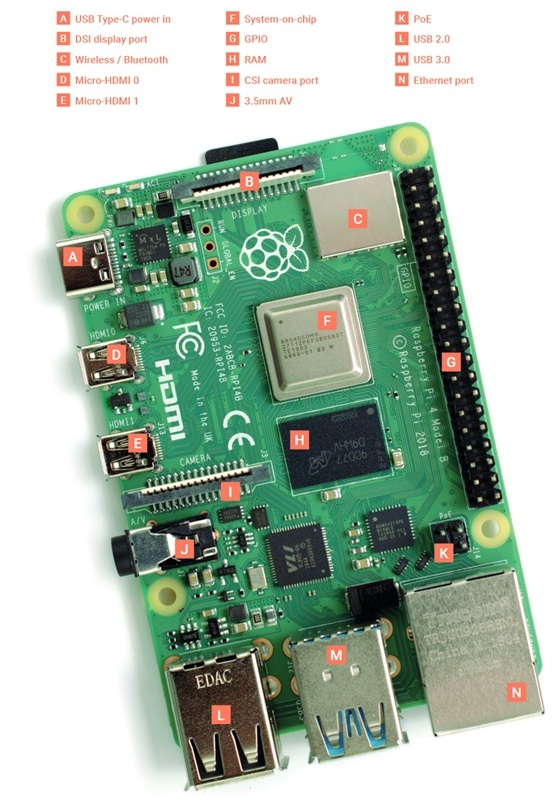
\includegraphics[scale=1.3]{raspberryPi.jpg}
	\caption{Raspberry Pi 4 Model B}
	\label{fig:raspberry4B}
\end{figure}

Архитектура Raspberry Pi, как и любого современного компьютера, основана на взаимодействии специализированных компонентов, каждый из которых выполняет строго определённые функции. Ключевым элементом системы является система на кристалле (System-on-Chip, SoC), расположенная в центральной части платы под металлическим теплораспределительным корпусом, что показано на рисунке \ref{fig:soc}. 

\begin{figure}[H]
	\centering
	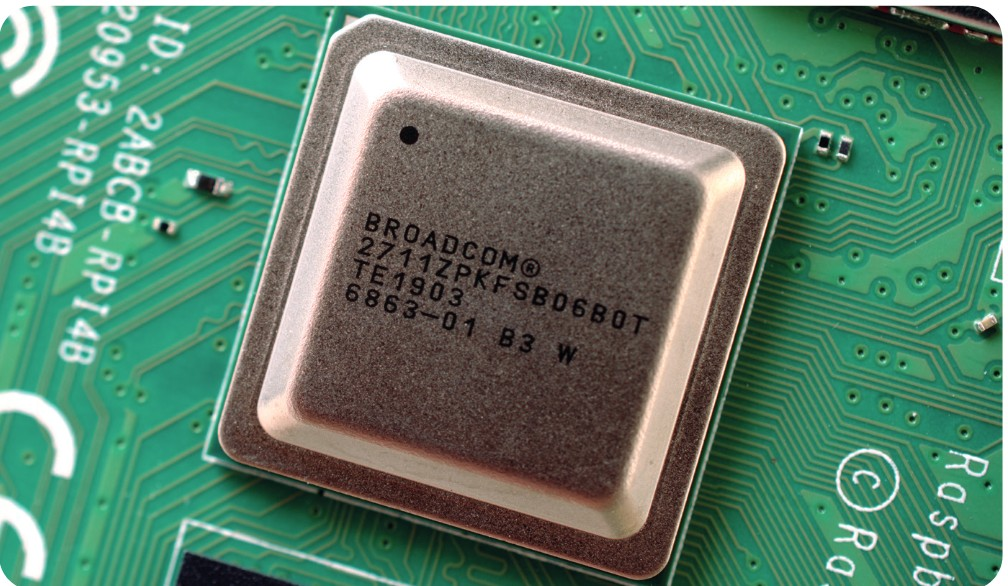
\includegraphics[scale=0.9]{systemOnChip.jpg}
	\caption{Raspberry Pi’s system-on-chip (SoC)}
	\label{fig:soc}
\end{figure}

Концепция "системы на кристалле" подразумевает интеграцию всех основных вычислительных блоков в единый полупроводниковый компонент. В состав SoC входят центральный процессор (CPU), выполняющий основные вычисления, графический процессор (GPU), отвечающий за обработку визуальных данных, а также набор вспомогательных контроллеров и интерфейсных модулей. Такая архитектура обеспечивает компактность, энергоэффективность и высокую степень интеграции компонентов, что особенно важно для встраиваемых систем. На рисунке \ref{fig:soc} чётко видно расположение данного компонента относительно других элементов платы, включая модули оперативной памяти и периферийные интерфейсы.

Для работы вычислительной системы необходима память разных типов. Рядом с системой на кристалле (SoC) расположен модуль оперативной памяти (RAM) - компактный черный чип квадратной формы смотрите рисунок \ref{fig:ram}.

\begin{figure}[H]
	\centering
	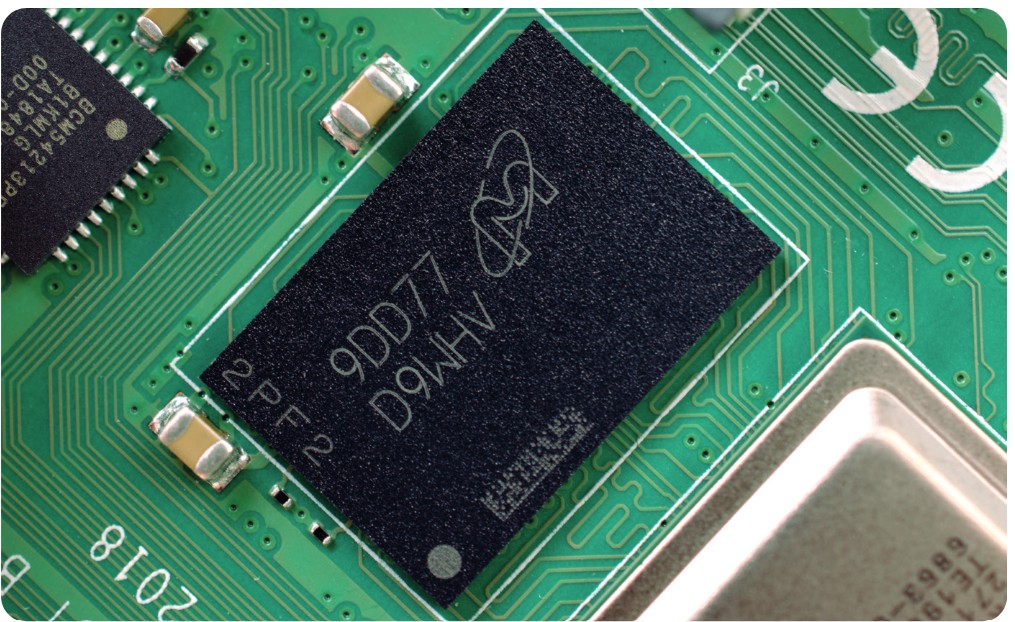
\includegraphics[scale=0.9]{ram.jpg}
	\caption{Raspberry Pi’s random access memory (RAM)}
	\label{fig:ram}
\end{figure}

Оперативная память временно хранит данные и команды, с которыми процессор работает в текущий момент. При этом все изменения сохраняются только при записи на microSD-карту. Эти два компонента представляют принципиально разные типы памяти: энергозависимую RAM, которая теряет данные при отключении питания, и энергонезависимую память microSD, сохраняющую информацию после выключения устройства.


В правом верхнем углу платы расположен радиомодуль, скрытый под металлическим экраном смотрите рисунок \ref{fig:radio_module}), который обеспечивает беспроводную связь Raspberry Pi.

\begin{figure}[H]
	\centering
	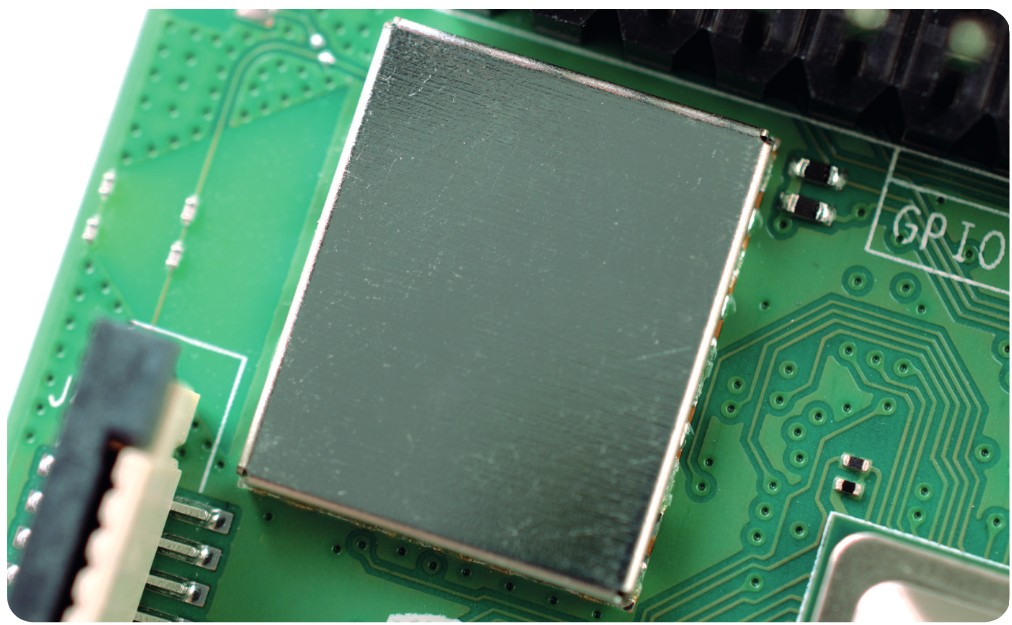
\includegraphics[scale=0.8]{radioModule.jpg}
	\caption{Raspberry Pi’s radio module}
	\label{fig:radio_module}
\end{figure}

Этот модуль объединяет два ключевых компонента: Wi- Fi-адаптер для подключения к беспроводным сетям и Bluetooth-радио для соединения с периферийными устройствами (такими как мыши и клавиатуры) и обмена данными с умными устройствами, включая датчики и смартфоны. Металлический экран выполняет важную функцию экранирования радиопомех, обеспечивая стабильную работу беспроводных интерфейсов.


В нижней части платы расположен USB-контроллер (черная микросхема в пластиковом корпусе), который управляет работой четырех USB-портов. Рядом с ним находится компактный сетевой контроллер, отвечающий за функционирование Ethernet-порта. В левом верхнем углу платы, непосредственно над разъемом питания USB Type-C, размещена интегральная схема управления питанием (PMIC) смотрите рисунок \ref{fig:pmic}.

\begin{figure}[H]
	\centering
	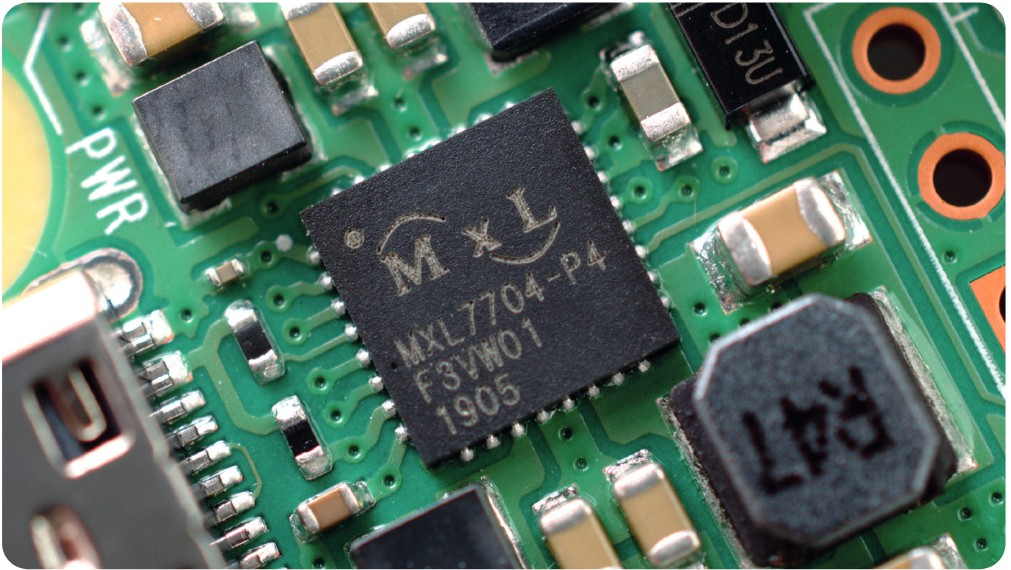
\includegraphics[scale=0.9]{pmic.jpg}
	\caption{Raspberry Pi’s power management integrated circuit (PMIC)}
	\label{fig:pmic}
\end{figure}

Этот критически важный компонент выполняет преобразование входного напряжения от источника питания в стабильные уровни, необходимые для корректной работы всех элементов Raspberry Pi. PMIC обеспечивает надежное электропитание процессора, оперативной памяти и периферийных устройств, поддерживая стабильность работы системы в различных режимах эксплуатации.

На плате Raspberry Pi расположены четыре порта Universal Serial Bus (USB), которые можно увидеть в центральной и правой части нижнего края рисунок \ref{fig:usb}.

\begin{figure}[H]
	\centering
	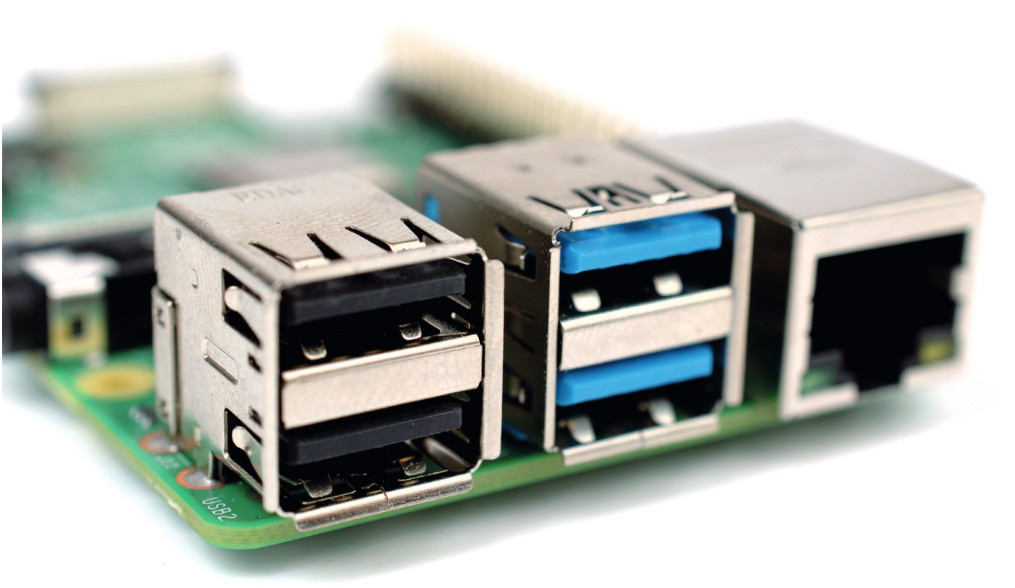
\includegraphics[scale=0.9]{usb.jpg}
	\caption{Raspberry Pi’s USB ports}
	\label{fig:usb}
\end{figure}

Эти порты предназначены для подключения различных USB-устройств - от клавиатур и мышей до внешних накопителей и цифровых камер. В соответствии с рисунком \ref{fig:usb}, порты представлены в двух вариантах: стандартные USB 2.0 с черными внутренними компонентами и более быстрые USB 3.0 с синими компонентами, что позволяет одновременно работать как с устаревшими, так и с современными высокоскоростными устройствами.

На плате Raspberry Pi справа от USB-портов расположен Ethernet-разъём (рисунок \ref{fig:ethernet}), предназначенный для подключения к проводной сети.

\begin{figure}[H]
	\centering
	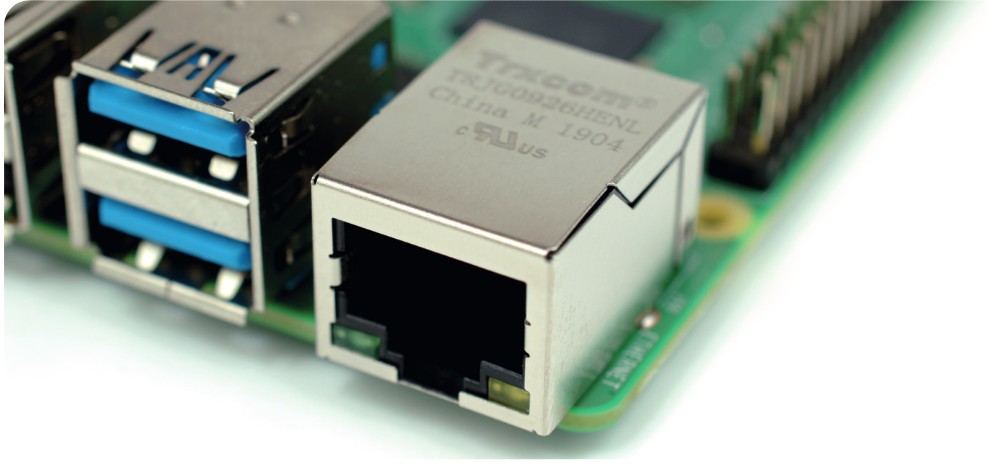
\includegraphics[scale=0.9]{ethernet.jpg}
	\caption{Raspberry Pi’s Ethernet port}
	\label{fig:ethernet}
\end{figure}

Этот стандартный сетевой интерфейс использует разъём типа RJ45, совместимый с обычными сетевыми кабелями. В нижней части порта, как показано на рисунке \ref{fig:ethernet}, расположены два светодиодных индикатора (LED), которые визуально отображают состояние сетевого подключения: активность передачи данных и наличие физического соединения. Такой интерфейс обеспечивает стабильное и высокоскоростное сетевое соединение, что особенно важно для серверных и сетевых применений Raspberry Pi.

На левой стороне платы Raspberry Pi, чуть выше USB-портов, расположен комбинированный 3.5 мм аудио-видео разъём (рисунок \ref{fig:jack}).

\begin{figure}[H]
	\centering
	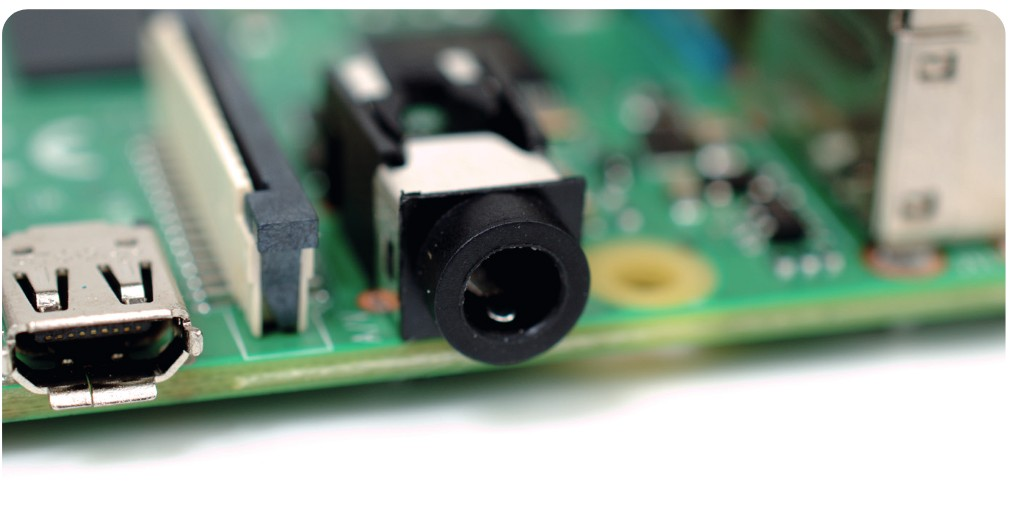
\includegraphics[scale=0.9]{jack.jpg}
	\caption{Raspberry Pi’s 3.5 mm AV jack}
	\label{fig:jack}
\end{figure}

Основное его назначение — вывод аналогового аудиосигнала, при этом подключение к активным колонкам обеспечивает лучшее качество звука, чем использование наушников. Кроме того, через этот разъём возможна передача аналогового видеосигнала (композитного видео) на телевизоры и проекторы при использовании специального TRRS-кабеля (tip-ring-ring-sleeve). Такой функционал делает данный интерфейс универсальным решением для мультимедийных применений.

Над комбинированным 3.5 мм аудио-видео разъёмом расположен специализированный интерфейс Camera Serial Interface (CSI) с пластиковым фиксатором (рисунок \ref{fig:camera}).

\begin{figure}[H]
	\centering
	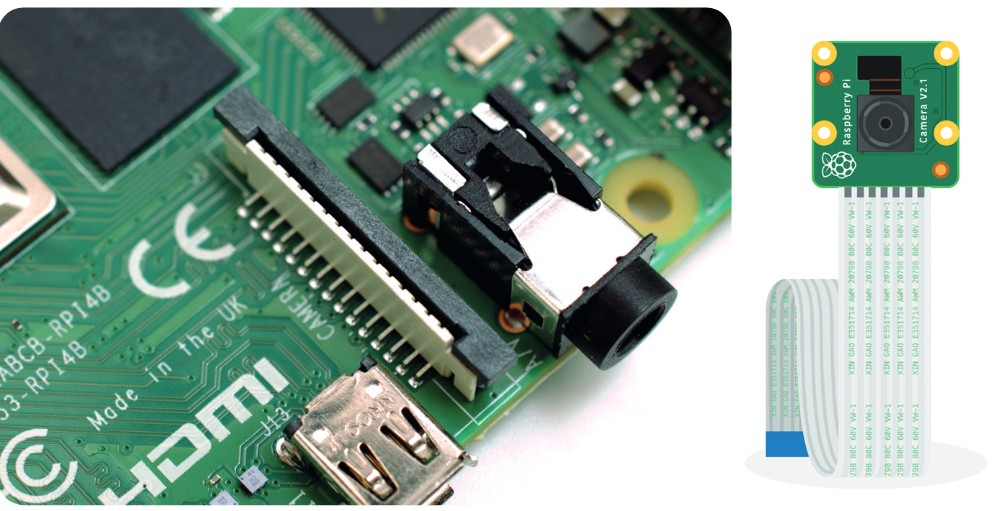
\includegraphics[scale=0.9]{camera.jpg}
	\caption{Raspberry Pi’s camera connector}
	\label{fig:camera}
\end{figure}

Этот разъём предназначен для подключения официального модуля камеры Raspberry Pi Camera Module, который подробно рассматривается в главе 8 настоящего руководства. Особенностью данного интерфейса является использование последовательного протокола передачи данных, оптимизированного для работы с цифровыми камерами. Пластиковая защёлка обеспечивает надёжное соединение с кабелем камеры, предотвращая случайное отсоединение.


В верхней части левого края платы расположены micro-HDMI разъемы (рисунок \ref{fig:microHDMI}) - компактные версии стандартных HDMI-интерфейсов.

\begin{figure}[H]
	\centering
	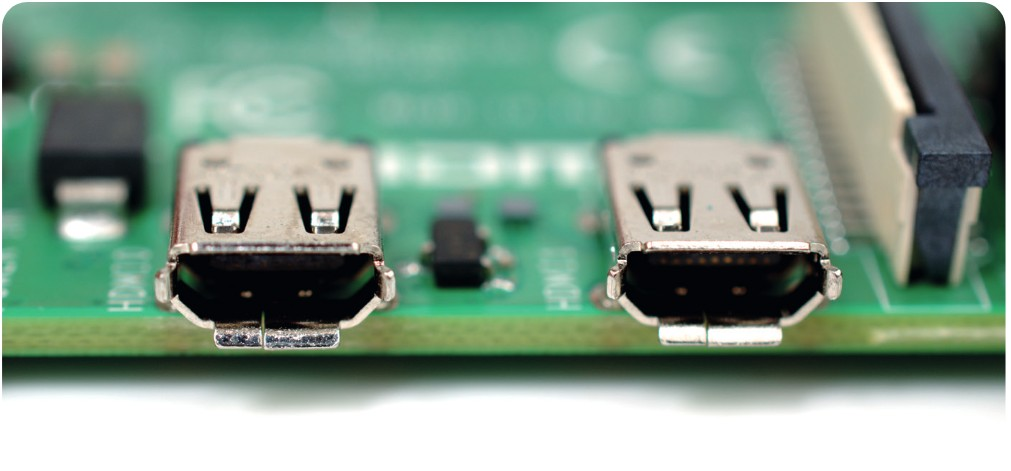
\includegraphics[scale=0.8]{microHDMI.jpg}
	\caption{Raspberry Pi’s micro-HDMI ports}
	\label{fig:microHDMI}
\end{figure}

Как видно на рисунке \ref{fig:microHDMI}, данные порты обеспечивают передачу цифровых аудио и видеосигналов высокой четкости, что позволяет подключать Raspberry Pi к одному или двум внешним устройствам отображения (мониторам, телевизорам или проекторам). Особенностью micro-HDMI является сохранение всех функциональных возможностей полноразмерного HDMI-интерфейса при существенно меньших габаритах разъема.


В верхней части платы, над HDMI-портами, расположен разъём питания USB Type-C (рисунок \ref{fig:typeC}).

\begin{figure}[H]
	\centering
	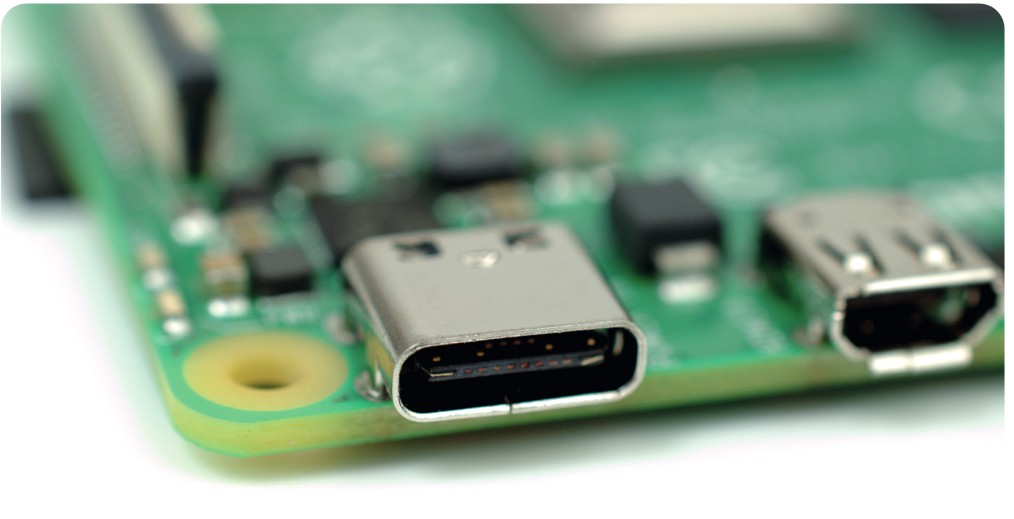
\includegraphics[scale=0.8]{typeC.jpg}
	\caption{Raspberry Pi’s USB Type-C power port}
	\label{fig:typeC}
\end{figure}

Данный интерфейс, широко распространённый в современных мобильных устройствах, служит для подключения Raspberry Pi к источнику электропитания. Как показано на рисунке \ref{fig:typeC}, этот компактный разъём обеспечивает надёжное соединение и позволяет использовать различные источники питания. Однако для стабильной работы системы, особенно при высокой нагрузке, рекомендуется применять официальный блок питания Raspberry Pi, специально разработанный для данной платформы и обеспечивающий необходимые параметры тока и напряжения.


В верхней части платы расположен специализированный разъём Display Serial Interface (DSI) (рисунок \ref{fig:display}), который внешне напоминает разъём для камеры, но функционально является его противоположностью.

\begin{figure}[H]
	\centering
	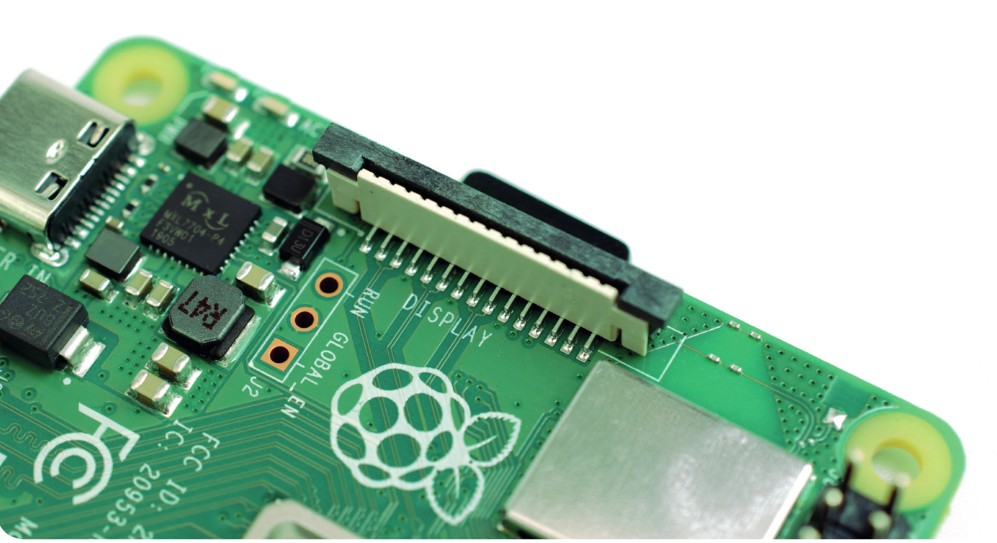
\includegraphics[scale=0.8]{display.jpg}
	\caption{Raspberry Pi’s USB Type-C power port}
	\label{fig:display}
\end{figure}

Как показано на рисунке \ref{fig:display}, данный интерфейс предназначен исключительно для подключения официального сенсорного дисплея Raspberry Pi. Особенностью DSI-разъёма является использование последовательного протокола передачи видеоданных, оптимизированного для работы с дисплеями. Пластиковый фиксатор обеспечивает надёжное соединение с дисплейным модулем, предотвращая случайное отсоединение кабеля. Этот интерфейс позволяет реализовать компактные решения с сенсорным вводом без использования дополнительных периферийных подключений.

На правой границе платы расположен 40-контактный GPIO-разъём (General-Purpose Input/Output), представляющий собой два параллельных ряда металлических контактов (рисунок \ref{fig:gpio}).

\begin{figure}[H]
	\centering
	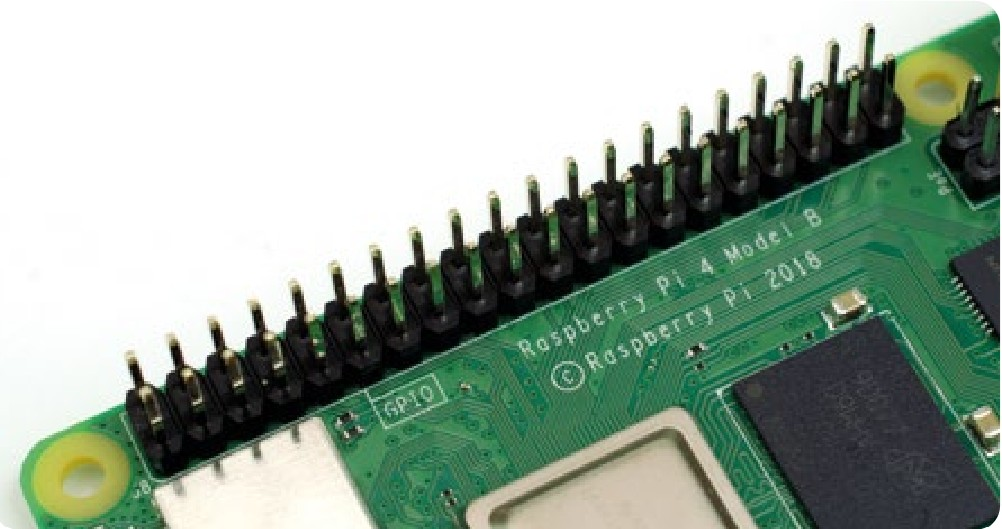
\includegraphics[scale=0.8]{gpio.jpg}
	\caption{Raspberry Pi’s GPIO header}
	\label{fig:gpio}
\end{figure}

Как показано на рисунке \ref{fig:gpio}, данный интерфейс обеспечивает возможность подключения широкого спектра внешних устройств - от простых электронных компонентов (светодиодов, кнопок) до сложных датчиков и измерительных приборов. Функциональные возможности GPIO-разъёма подробно рассматриваются в главе 6 настоящего руководства.

Непосредственно под GPIO-разъёмом, со смещением влево, расположен дополнительный 4-контактный интерфейс (рисунок \ref{fig:gpio}), предназначенный для подключения модуля PoE HAT (Power over Ethernet). Как видно на рисунке \ref{fig:gpio}, данный модуль позволяет организовать электропитание Raspberry Pi через Ethernet-кабель, что обеспечивает альтернативу стандартному питанию через USB Type-C разъём и особенно востребовано в сетевых и встраиваемых решениях.

На обратной стороне платы Raspberry Pi, прямо под дисплейным разъёмом, расположен слот для microSD-карты (рисунок \ref{fig:microSd}).

\begin{figure}[H]
	\centering
	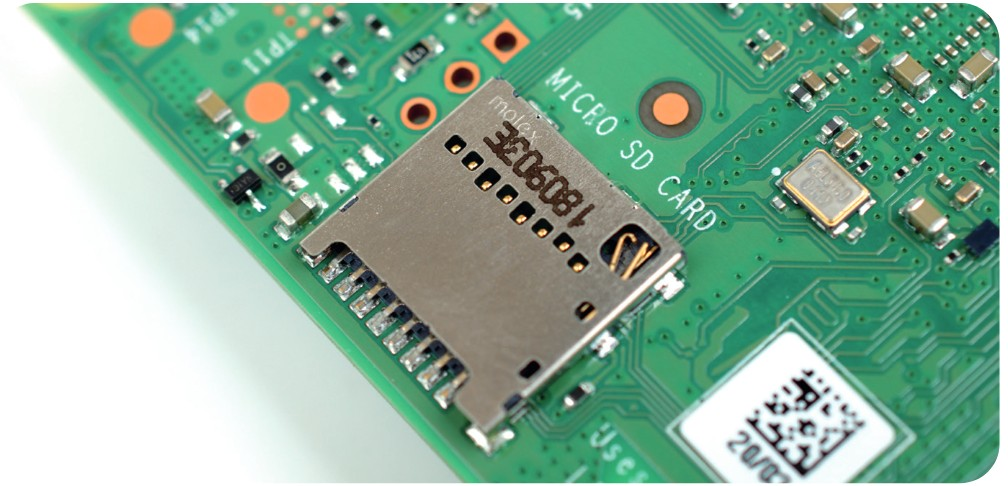
\includegraphics[scale=0.8]{microSd.jpg}
	\caption{Raspberry Pi’s microSD card connector}
	\label{fig:microSd}
\end{figure}

Этот слот служит основным хранилищем системы - в него вставляется карта памяти с операционной системой, пользовательскими файлами и установленными программами. В отличие от оперативной памяти, данные на microSD-карте сохраняются после выключения питания. Использование съёмного носителя обеспечивает гибкость при смене операционной системы или восстановлении данных \cite{RaspberryPi}.
\newpage
